\chapter{Effective Testing}
\label{chap:Effective_Testing}
This chapter explains the testing strategy of the Sequence library. The start
shows the instruments already available from the Kolibri Web UI Toolkit and how
we used them. After that, we focus on the testing table - the core of
the implemented testing framework during this project. The end of the chapter
discusses some advanced concepts regarding property-based testing.

\section{Motivation}
\label{sec:Motivation}
When implementing a library, testing is an essential task. With the constant
increase of functionalities, the number of tests also grows. Therefore, it
brings many benefits to implementing tests in a standardized and generalized
way. This leads to a robust and leakless testing framework and, thus, a solid
code base. We called our implementation of this generalization "testing table".
An explanation in detail follows in section~\ref{sec:Testing Table}. \\
Such a testing strategy has significant advantages. The following
non-concluding list shows an excerpt of the most important:

\begin{itemize}
  \item{Ensuring high code quality}
  \item{Avoid incompleteness - prevent missing test cases}
  \item{Prevent code duplication}
  \item{Less effort in writing tests}
  \item{Better overview of the code base}
  \item{Easier to understand test cases}
\end{itemize}

The generalization of testing is possible for functions that meet similar
constraints. This enables to write configurations for such functions under
test, which the testing framework then checks against certain predefined rules.
Suppose a new particular case, probably a bug, is discovered during the
development that also affects existing implementations. Then a new test
covering this issue is added to the rules, which runs automatically against all
testing configurations.

\section{Kolibri Testing Framework}
\label{sec:Kolibri Test Framework}
The Kolibri already provides a testing framework. We extended the framework
with some iterable specific functionalities for easier testing of our
implementations.

\subsection{Parts of the Framework}
\label{sub:Parts of the Framework}
The test suite is the core element of the testing framework. Typically, a
test suite includes several tests, whereas a testing framework can consist of
several suites. Executing the test suites generates a test report in HTML.
An example of such a summary report shows figure~\ref{fig:test_report}:

\begin{figure}[H]
    \centering
    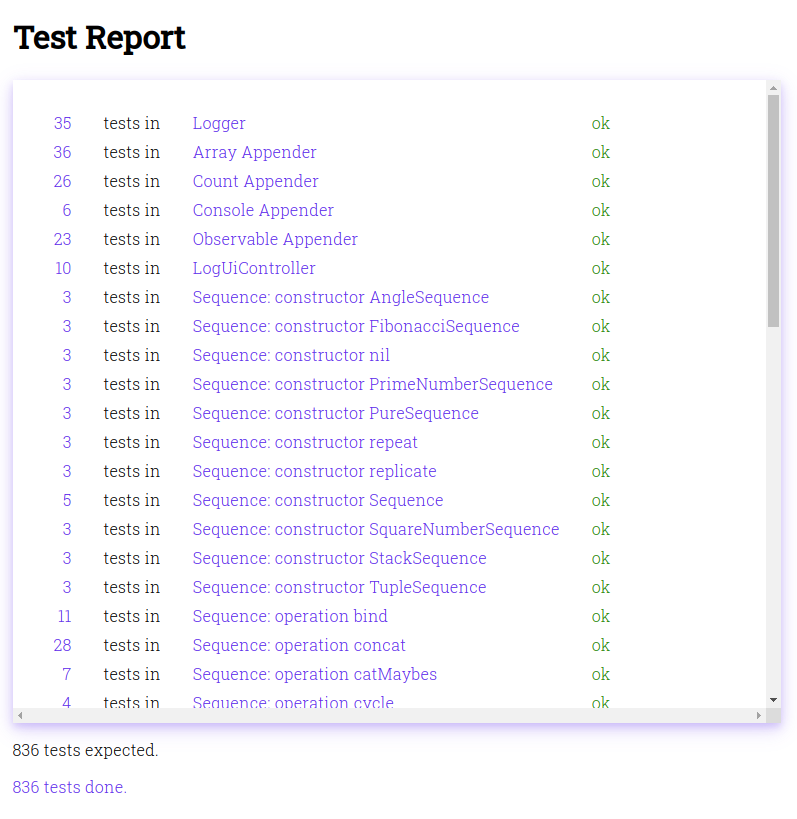
\includegraphics[width=0.8\textwidth]{mainmatter/pictures/test_report.png}
    \caption{Example test report}
    \label{fig:test_report}
\end{figure}


To demonstrate how to work with the test suite, examine the following
listing~\ref{lst:testsuit_demo}:

\begin{lstlisting}[
  style=ES6, 
  caption=TestSuite demonstration,
  label={lst:testsuit_demo}
  ]
const suite = TestSuite("The truth");
suite.add("true is really true", assert => {
  assert.is(true, true);
});
suite.run();
\end{lstlisting}

Description of the functionalities: 

\begin{itemize}
  \item{|TestSuite|: A |TestSuite| contains the test cases and is identified by a
    name. This name represents the suite on the summary page in 
  figure~\ref{fig:test_report} when executing.}
  \item{|run|: executes all tests containing the |TestSuite|.}
  \item{|add|: A function for including a test case into |TestSuite|. Its
      parameters are a string |name| and a callback which provides the test.}
\end{itemize}

\subsection{Additional Assertions}
\label{sub:Additional Assertions}

Assert functions in the Kolibri testing framework execute tests by comparing
two values and store the result in a summary collection of the test suite.
Listing~\ref{lst:testsuit_demo} shows the comparison of two booleans using the
|assert.is(...)| function.
This function compares an |actual| and an |expected| value. The references of
these two values must match. Otherwise, the test fails.

\subsubsection{Assertion}
\label{subsub:Assertion for Iterables}
Comparing iterables is slightly more complicated. For this reason, we extended
the testing framework with an additional assert function that compares two
arbitrary iterables. Listing~\ref{lst:iterableEq} shows the usage of this
function called |iterableEq|:

\begin{lstlisting}[
  style=ES6, 
  caption=Usage of iterableEq,
  label={lst:iterableEq}
  ]
testSuite.add("demo iterableEq", assert => {
  const sequence = Sequence(0, x => x < 2, x => x +1);

  assert.iterableEq(sequence, [0,1]);
  assert.iterableEq(sequence, Pair(0)(1));
  assert.iterableEq(sequence, Range(1));
});  
\end{lstlisting}

The implementation of |iterableEq| is suitable for any two iterables.
Listing~\ref{lst:impl_iterableEq} shows the implementation of |iterableEq|:

\begin{lstlisting}[
  style=ES6, 
  caption=Implementation of iterableEq,
  label={lst:impl_iterableEq}
  ]
// test.js
...
iterableEq: (actual, expected, maxElementsToConsume = 1_000) => { *'\label{line:signature_iterableEq}'*

    if (actual[Symbol.iterator]   === undefined) error("..."); *'\label{line:check_iterable}'*
    if (expected[Symbol.iterator] === undefined) error("...");

    const actualIt     = actual[Symbol.iterator]();
    const expectedIt   = expected[Symbol.iterator]();

    let iterationCount = 0;
    let testPassed     = true;
    let message        = "";

    while (true) {
     const { value: actualValue,   done: actualDone  } = actualIt.next();
     const { value: expectedValue, done: expectedDone } = expectedIt.next();

     const oneIteratorDone      = actualDone || expectedDone;
     const bothIteratorDone     = actualDone && expectedDone;
     const tooManyIterations    = iterationCount > maxElementsToConsume;

     if (bothIteratorDone) break;*'\label{line:check_iterable2}'*
     if (oneIteratorDone) {
         testPassed = false;
         message    = '...'
         break;
     }
     if (tooManyIterations) {
         message    = '...'
         testPassed = false;
         break;
     }
     if (actualValue !== expectedValue) {
         testPassed = false;
         message    = '...'
         break;
     } *'\label{line:check_iterable3}'*

     iterationCount++;
    }
    if (!testPassed) error(message);
    results.push(testPassed);*'\label{line:write_result_to_summary}'*
    messages.push(message);
}
\end{lstlisting}
Since an iterable can be endless, |iterableEq| defines a default maximum
iteration amount on line~\ref{line:signature_iterableEq}
(|maxElementsToConsume|).  This is handy because it is often the case that an
iterable runs infinitely when something goes wrong. If an iterable exceeds this
limit, the test fails.\\
The implementation checks on line~\ref{line:check_iterable} if both values are
iterable. If this is the case, it compares the iterables using a |while| loop:
Lines~\ref{line:check_iterable2} to~\ref{line:check_iterable3} check the
equality for each iteration - if one iterator has fewer elements, it took
too many iterations or the values at the same position are not equal, the test
fails. \\ 
On line~\ref{line:write_result_to_summary}, the
test stores the result in the summary collection of the corresponding test
suite.
\newline

\subsubsection{Assertion for Exceptions}
\label{subsub:Assertion for Exceptions}
Another extension for the testing framework is the |assert.throws| function. It
is often the case that functions must throw an exception in a specific
situation. For example, when looking for the maximum in an empty iterable.
|max| throws an exception in this case. Therefore, testing the function's
behaviour in error cases is also required. For this purpose,
listing~\ref{lst:impl_throws} shows the implementation of |assert.throws|:

\begin{lstlisting}[
  style=ES6, 
  caption=Implementation of assert.throws,
  label={lst:impl_throws}
  ]
// test.js
...
throws: (functionUnderTest, expectedErrorMsg = "") => {
     let testResult    = false;
     let message       = "";
     const hasErrorMsg = expectedErrorMsg !== "";

     try {
         functionUnderTest();*'\label{line:functionToTest}'*
         message = "Did not throw an error!";
         if (hasErrorMsg) {
             message += ` Expected: '${expectedErrorMsg}'`;
         }
         error(message);
     } catch (e) {
         testResult = true;

         if (hasErrorMsg) {
             testResult = expectedErrorMsg === e.message;
         }
     }
     results .push(testResult);
     messages.push(message);
 }
 ...
\end{lstlisting}


Line~\ref{line:functionToTest} calls the function under test. As expected, this
function should throw an exception that is caught in the catch block. If this
is the case, the test is successful. Otherwise, the test fails and a
corresponding error message is stored.

\section{Testing Table}
\label{sec:Testing Table}
The testing table enables generalizing test cases for operations of the
Sequence library. Each function under test must provide a configuration for the
testing framework.

The architecture consists of three main parts:
\begin{enumerate}
  \item{a table containing all testing functions}
  \item{configuration objects to define test properties}
  \item{a function |addToTestingTable| including all tests from the testing
    table into a given test suite}
\end{enumerate}

Each constructor and operator of the Sequence library has its configuration
that specifies the test behaviour. Likewise, each has its |TestSuite|. 

\subsection{Configuring the Testing Table}
\label{sub:Configuring the Testing Table}

In order to test operators and constructors using the testing table, it is
necessary to implement a test configuration.
Listing~\ref{lst:config_reduce} shows the testing file of the function |reduce|. 
Lines~\ref{line:start_test_config} to \ref{line:end_test_config} define the test 
configuration. The testing table does not handle special cases. Those follow 
later in the same file from line~\ref{line:additional_test_cases} on:

\begin{lstlisting}[
  style=ES6, 
  caption=Test configuration reduce,
  label={lst:config_reduce}
  ]
const testSuite = TestSuite("Sequence: terminal operation reduce$");

addToTestingTable(testSuite)(*'\label{line:start_test_config}'*
  createTestConfig({*'\label{line:createTestConfig}'*
    name:      "reduce$",
    iterable:  () => newSequence(UPPER_SEQUENCE_BOUNDARY),
    operation: () => reduce$((acc, cur) => acc + cur, 0),
    expected:  10,
    evalFn:    expected => actual => expected === actual,
    excludedTests: [TESTS.TEST_CB_NOT_CALLED_AFTER_DONE]
  })
);*'\label{line:end_test_config}'*

testSuite.add("test: special case", assert => {*'\label{line:additional_test_cases}'*
  // Given
  // When
  // Then
});

testSuite.run();
\end{lstlisting}

On line~\ref{line:createTestConfig}, the function |createTestConfig|  sets
default values of configuration properties to simplifying the code.

The table~\ref{tab:testing_table} shows the available configuration 
properties and their purpose:

\begin{table}[H]
  \center
  \begin{tabular}{ l m{10cm} c}
    \textbf{Property} & \textbf{Description} & \textbf{Required}\\
    \hline
    |name|            & The name of the test for meaningful 
                      reporting messages. 
                    & y 
                    \\ 
    |iterable|        & A function that constructs a new iterable to apply the 
                      operation to. 
                    & y 
                    \\  
    |expected|        & The expected result of the operation applied to the iterable
                      defined in property |iterable|.
                    & 
                    y  \\ 
    |excludedTests|   & An optional array of testing functions to exclude tests
                      in the testing table. 
                    & n 
                    \\
    |operation|       & The operation to test. |param| is passed as an argument
                      to it
                     (leave this empty for constructor 
                      tests since they do not take an inner iterator). 
                    & n 
                    \\
    |param|           & A parameter passed to this |operation|. If it is a
                      function, some extra tests will be performed. 
                    & n
                    \\ 
    |invariants|      & An optional array of |InvariantCallback|. The invariant 
                      must hold tests against different lists. 
                    & n
                    \\
    |evalFn|          & An optional function that compares the |expected| and 
                      the |actual| values. The default is |iterableEq|.
                    & n 
                    \\
  \end{tabular}
  \caption{Properties of the configuration object}
\label{tab:testing_table}
\end{table}

\subsection{The Table}
\label{sub:The Table}
The testing table is just an array (table) containing test objects.
Listing~\ref{lst:testing_table} shows the implementation:

\begin{lstlisting}[
  style=ES6, 
  caption=Testing table,
  label={lst:testing_table}
  ]
const testingTable = [
  { name: TESTS.TEST_SIMPLE,                   test: testSimple},
  { name: TESTS.TEST_PURITY,                   test: testPurity},
  { name: TESTS.TEST_CB_NOT_CALLED_AFTER_DONE, test: testCBNotCalledAfterDone},
  { name: TESTS.TEST_PROTOTYPE,                test: testPrototype},
  { name: TESTS.TEST_INVARIANTS,               test: testInvariants},
  { name: TESTS.TEST_ITERATE_MULTIPLE_TIMES,   test: testIterateMultipleTimes},
];
\end{lstlisting}

An object in the table includes two properties:
\begin{itemize}
\item{A string representing its name. The name is important for displaying an 
  accurate error message if the test fails}
\item{A function to test a specific behaviour}
\end{itemize}

Each function of the testing table expects as argument a test configuration
object of type |SequenceTestConfigType|. Listing~\ref{lst:test_simple} presents
exemplary the implementation of |testSimple|:

\begin{lstlisting}[
  style=ES6, 
  caption=Implementation test simple,
  label={lst:test_simple}
  ]
/**
 * @type {
 *             (config: SequenceTestConfigType)
 *          => (assert: AssertType)
 *          => void
 *       }
 */
const testSimple = config => assert => {
  const { iterable, operation, evalFn, expected, param } = config;*'\label{line:test_config_destructuring}'*
  const baseIterable = iterable(); *'\label{line:test_config_iterable}'*
  const operated     = operation(param)(baseIterable);*'\label{line:test_config_operated}'*
  evaluate(expected, operated, assert, evalFn);*'\label{line:test_config_eval}'*
};
\end{lstlisting}

The function |simpleTest| examines whether an operation correctly processes a typical use case.
For this purpose, it executes the following tasks: 
\begin{itemize}
  \item{Line~\ref{line:test_config_iterable} shows the invocation of the
      function |iterable| to create an iterable for further use.}
  \item{Line~\ref{line:test_config_operated} executes the operation to test on
      the previously obtained iterable by passing the required parameters.
      |param| is optional and can, therefore, also be left empty. This covers
      cases where operations need to be parametrized (like |map|, which takes a
      mapping function).}
  \item{Line~\ref{line:test_config_eval} calls a function |evaluate|, which
      then calls the passed function |evalFn|, comparing the |actual| and
      |expected| values. This gives the possibility to evaluate iterables or
      sequences containing more complex values or if the output of an operation
      is not an iterable anymore (as, for example, with |reduce|). If |evalFn| is
    undefined, the fallback function |iterableEq| is used, comparing two
  iterables which section~\ref{sub:Additional Assertions} explains.} 
\end{itemize}

The testing table includes test-functions to examine the following behaviours of
implementations of the Sequence library:

\begin{itemize}
  \item{\textbf{testSimple} checks if a typical case works properly.}
  \item{\textbf{testPurity} checks if an operator makes some side effects.}
  \item{\textbf{testCBNotCalledAfterDone} checks if a given callback of an
    operator will be called when the iterable is exhausted.}
  \item{\textbf{testPrototype} checks if the |SequencePrototype| is set.}
  \item{\textbf{testInvariants} checks if an invariant holds by applying different parameters.}
  \item{\textbf{testIterateMultipleTimes} checks if an iterable produces the same output twice.}
\end{itemize}

\subsection{Running the Testing Table}
\label{sub:Running the Testing Table}
|addToTestingTable| must be called for each configuration to be tested by the
testing table. It runs each test with the given configuration
(line~\ref{line:add_to_testsuite}). Some tests do not make sense for all
functions of the Sequence library - since |addToTestingTable| runs all tests by
default, it must provide an option to exclude such tests. For
example, if an operation has no callback, the check of its side effect is
useless.

Line~\ref{line:filtering_tests} filters out tests excluded by the
configuration:
\begin{lstlisting}[
  style=ES6, 
  caption=Implementation of addToTestingTable,
  label={lst:impl_addToTestingTable}
  ]
export { addToTestingTable }
...
/**
 * @type {
 *       (testSuite: TestSuiteType)
 *    => (config: SequenceTestConfigType)
 *    => void
 * }
 */
const addToTestingTable = testSuite => config => {
  const { excludedTests } = config;

  testingFunctions
    .filter (({ name })        => !excludedTests.includes(name)) *'\label{line:filtering_tests}'*
    .forEach(({ name, test })  => 
         testSuite.add(`${name}: ${config.name}`, test(config)));*'\label{line:add_to_testsuite}'*
};
\end{lstlisting}


\section{Testing based on Properties}
\label{sec:Testing based on Properties}
John Huges and Carl Claessen wrote the following sentence in the paper
"Quickcheck, A Lighweight Tool for Random Testing of Haskell Programms":
\textit{
Despite anecdotal evidence that functional programs require somewhat less
testing (`Once it type-checks, it usually works'), in practice it is still a 
major part of functional program development}~\cite{quickcheck_hughes}.
If these programming icons claim it takes many tests even in a strongly typed 
language, how many does it take in JavaScript? Of course, enough.

\subsection{Invariant Testing}
\label{sub:Invariant Testing}
Invariant tests add another layer of verification to ensure the correctness of
the Sequence library. Some aspects of this testing are leaned on the Quickcheck
approach of the paper mentioned before. We concentrated on only some essential
parts since implementing the whole Quickcheck framework would compared to the
effort not bring enough benefits for this work.
\newline
The test configuration object contains a property |invariant|. It allows
defining of some invariants, which are tested against different iterables.
Quickcheck does this with randomly generated data. Our data is fixed and
includes a mix of special cases.
\newline
Line~\ref{line:reverse_law} in listing~\ref{lst:test_config_reverse} defines
the invariants of |reverse|. This statement defines that an iterable must be 
equal to the original when reversed two times:

\begin{lstlisting}[
  style=ES6, 
  caption=Test configuration reverse,
  label={lst:test_config_reverse}
  ]
const testSuite = TestSuite("Sequence: operation reverse$");

addToTestingTable(testSuite)(
  createTestConfig({
    name:      "reverse$",
    iterable:  () => newSequence(UPPER_SEQUENCE_BOUNDARY),
    operation: () => reverse$,
    expected:  [4, 3, 2, 1, 0],
    invariants: [
      *'\colorbox{code-highlight}{it => reverse$(reverse$(it)) ["=="] (it), }'* *'\label{line:reverse_law}'*
    ]
  })
);

testSuite.run();
\end{lstlisting}
The testing table contains a test function |testInvariants|.
Listing~\ref{lst:invariant_penetration} defines that function:

\begin{lstlisting}[
  style=ES6, 
  caption=Implementation invariant penetration,
  label={lst:invariant_penetration}
  ]
/**
 * Applies a series of lists to a given invariant.
 * @template _T_
 * @type {
 *            (invariants: InvariantCallback)
 *         => (assert: AssertType)
 *         => void
 *       }
 */
const invariantPenetration = invariant => assert => {
  const testingLists = [ *'\label{line:list_of_parameters}'*
    // edge case
    nil,                                                   
    // edge case, done calculated
    newSequence(1),                                        
    // typical number
    newSequence(3),                                        

    // no big iterable, needs extra test

    // edge case, done set explicitly
    PureSequence("testString"),                            
    // mixing types
    ['a', 'b', 'c', 1, 2, 3, Nothing, Just("testString")], 
    // iterable of iterables
    [PureSequence(1), newSequence(4), '#', "abc", 1]       
  ];

  for (const list of testingLists) {
    const result = invariant(list);
    assert.isTrue(result);
  }
};
\end{lstlisting}

Line~\ref{line:list_of_parameters} defines a list with several parameters of
type |Iterable|. Each parameter tests if the invariant of |reverse| holds. 
This enables testing many cases written in a few lines of code.

\subsubsection{An advanced Example}
\label{subsub:An advanced Example}
Listing~\ref{lst:lr_identity_mconcat} shows the definition of the identity law
for the function |<>| in Haskell which concatenates two lists:

\begin{lstlisting}[
  style=Haskell,
  caption=Left and right identity of <> in Haskell,
  label={lst:lr_identity_mconcat}
]
-- left identity
x <> mempty = x
-- right identity
mempty <> x = x
\end{lstlisting}

Listing~\ref{lst:lr_identity_mconcat} demonstrates that a list $x$ concatenated
with |nil|, the empty list, equals the original one. 
Besides |<>| there is also |mconcat|. |mconcat| allows flattening a list consisting
of further lists to a single list. This operation is often used and, therefore,
also exists in the Sequence library. As |<>|, |mconcat| is also
associative and a concatenation with the neutral element (the empty list)
has no influence on the result.\\ 
With the previously shown implementation of the invariant based testing, it
becomes possible to test these laws for |mconcat|.
Listing~\ref{lst:mconcat_invariant} shows the implementation of these
invariants in JavaScript:

\begin{lstlisting}[
  style=ES6, 
  caption=Invariants of mconcat,
  label={lst:mconcat_invariant}
  ]
addToTestingTable(testSuite)(
  createTestConfig({
    name:       "mconcat",
    iterable:   () => 
      toMonadicIterable([ newSequence(2), newSequence(2), newSequence(2) ]),
    operation:  () => mconcat,
    expected:   [0, 1, 2, 0, 1, 2, 0, 1, 2],
    invariants: [*'\label{line:mconcat_first_invariant}'*
      it => mconcat([nil, it]) ["=="] (it),
      it => mconcat([it, nil]) ["=="] (it),
      // ...
    ],*'\label{line:mconcat_second_invariant}'*
  })
)
\end{lstlisting}

Let us focus on lines~\ref{line:mconcat_first_invariant}-\ref{line:mconcat_second_invariant}.
The property |invariants| expect an array of functions. Each of these
functions represents a law. Therefore, the function injects an arbitrary
iterable called |it|, and the law must hold for it.

\subsection{Revealed Code Bugs: Discoveries through Testing during Development}
\label{sub:Revealed Code Bugs: Discoveries through Testing during Development}
As illustrated in the testing table section, a test case named
|TEST_CB_NOT_CALLED_AFTER_DONE| guarantees that a callback is not invoked once
an iterator is exhausted. This test arose from a bug during development
that it is expected for a callback not to be called after the iterator is used
up. Such occurrences could lead to program errors or unexpected behaviour.
Consequently, we implemented a test case addressing this scenario and added it
to the testing table. By adding just one more test, the entire Sequence library
could be examined for this behaviour, allowing for further improvements and
finding the same bug in other functions.\\
Another example concerns the behaviour of operators and operations when dealing
with empty iterables. When a test configuration provides an invariant,
it is automatically tested against the empty sequence. This is a powerful way
to ensure that invariants apply to all types of sequences.\\
Furthermore, another special test case is the |TEST_PURITY|, which ensures that
the state of an iterable is in the proper location. This safeguards against
unexpected side effects, promoting a more reliable program execution.

\subsection{Conclusion}
\label{sub:Conclusion}
When implementing large code bases, having a solid test framework is crucial.
Structured extension of the test suite during development leads to extensive
core functionality testing. Thus, the core of the library becomes even more
robust when the code base grows.
\newline
The standardization and generalization of tests using a testing table imply that
writing tests for new functionalities takes less time and ensures better
quality.
